\section{Shuffle Model for Graphs}
\label{sec:shuffle}
In this work, we apply the shuffle model to graph data to accurately estimate subgraph counts, such as triangles and 4-cycles. 
Section~\ref{sub:technical} explains our technical motivation. 
% the motivation of our approach. 
In particular, we explain why it is challenging to apply the shuffle model to graph data. 
Section~\ref{sub:wedge_shuffle} proposes a wedge shuffle technique to overcome the technical challenge. 

% \subsection{Technical Challenges}
\subsection{Our Technical Motivation}
\label{sub:technical}

\begin{figure}[t]
  \centering
  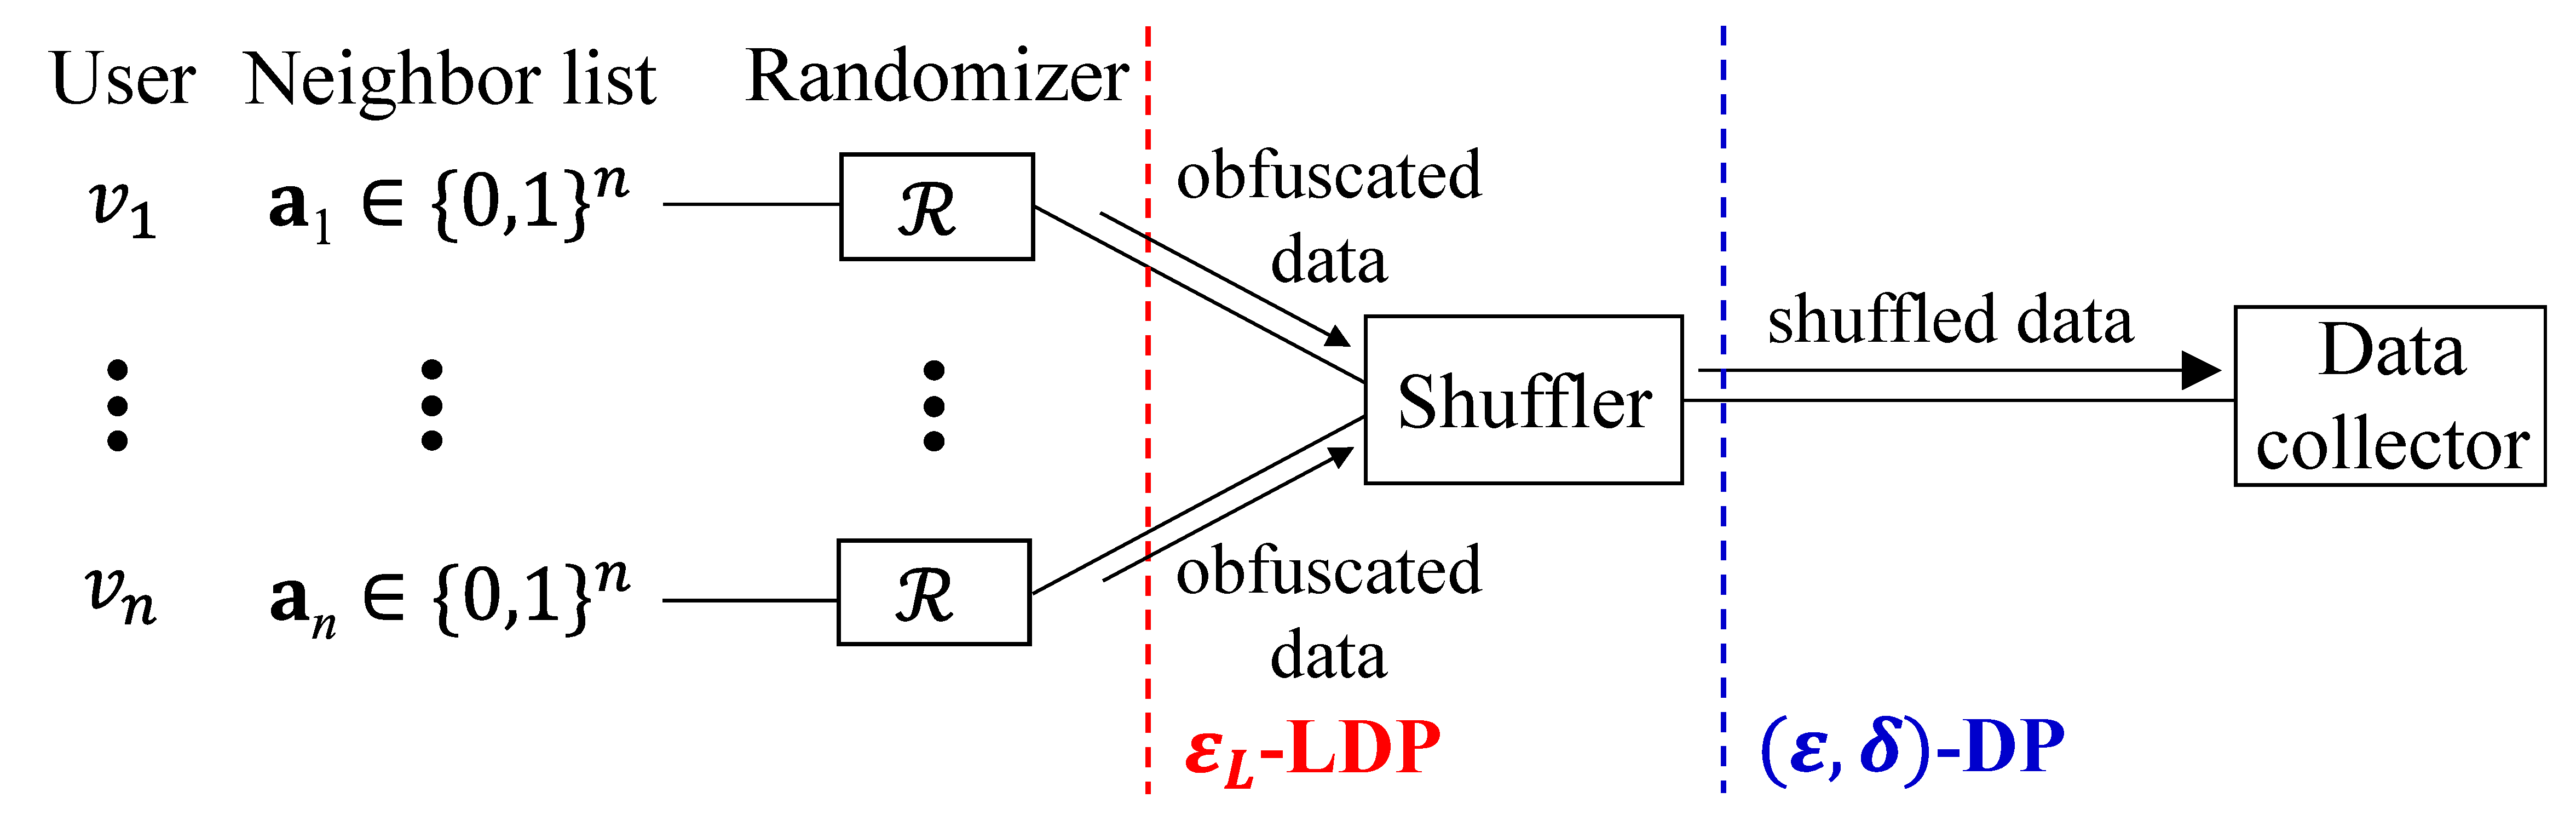
\includegraphics[width=0.99\linewidth]{fig/shuffle.pdf}
  \vspace{-2mm}
  \caption{Shuffle model for graphs. 
  %User $v_i$ calculates input data from her neighbor list $\bma_i$ and obfuscates the input data. 
  %The shuffler randomly shuffles the obfuscated data. 
  }
  \label{fig:shuffle_model}
\end{figure}

% the privacy-utility trade-off can be significantly improved 
% The privacy budget $\epsilon$ (hence the estimation error at the same value of $\epsilon$) can be dramatically reduced by introducing the shuffler. 
The shuffle model has been introduced to dramatically reduce the privacy budget $\epsilon$ (hence the estimation error at the same value of $\epsilon$) in tabular data \cite{Wang_PVLDB20} or 
% image data 
gradients 
\cite{Girgis_AISTATS21,Liu_AAAI21}. 
However, it is very challenging to apply the shuffle model to graph data analysis, as explained below. 

Figure~\ref{fig:shuffle_model} shows the shuffle model for graph data, where each user $v_i$ has her neighbor list $\bma_i \in \{0,1\}^n$. 
% The main reason for this 
The main challenge here 
% in the graph shuffle model 
is that 
% because 
the shuffle model uses a \textit{standard} definition of LDP for the local randomizer and that a neighbor list is \textit{high-dimensional data}, i.e., $n$-dim binary string. 
Specifically, LDP in Definition~\ref{def:LDP} requires any pair of inputs $x$ and $x'$ to be indistinguishable; i.e., 
the inequality (\ref{eq:LDP}) must hold for all pairs of possible inputs. 
Thus, if we use the entire neighbor list 
% (i.e., $n$-dim binary string) 
as input data (i.e., $\bma_i = x_i$ in Theorem~\ref{thm:shuffle}), 
% the standard LDP definition destroys 
either privacy or utility is destroyed for large $n$. 

To illustrate this, consider the following example. 
Assume that $n=10^5$ and $\delta=10^{-8}$. 
Each user $v_i$ applies 
% Warner's RR 
$\epsilon_0$-RR 
with $\epsilon_0=1$ to each bit of her neighbor list $\bma_i$. 
This mechanism is called the randomized neighbor list \cite{Qin_CCS17} and provides $\epsilon_0$-edge LDP. 
% which considers two neighbor lists that differ in one bit. 
However, the privacy budget $\epsilon_L$ in the standard LDP (Definition~\ref{def:LDP}) 
is extremely large -- by group privacy \cite{DP}, $\epsilon_L = n \epsilon_0 = 10^5$. 
Because 
$\epsilon_L$ 
% $n\epsilon$ 
is much larger than $\log (\frac{n}{16 \log (2/\delta)}) = 8.09$, we cannot use the privacy amplification result in Theorem~\ref{thm:shuffle}. 
This is evident from the fact that the shuffled data $y_{\pi(1)}, \ldots, y_{\pi(n)}$ are easily re-identified when $n$ is large. 
If we use 
% Warner's RR 
$\epsilon_0$-RR 
with $\epsilon_0 = \frac{1}{n}$, we can use the amplification result (as $\epsilon_L = n \epsilon_0 = 1$). 
However, it makes obfuscated data almost a random string and destroys the utility because $\epsilon_0$ is too small. 

In this work, we address this issue by introducing a basic technique, which we call \textit{wedge shuffling}. 

\subsection{Our Approach: Wedge Shuffling}
\label{sub:wedge_shuffle}

\begin{figure}[t]
  \centering
  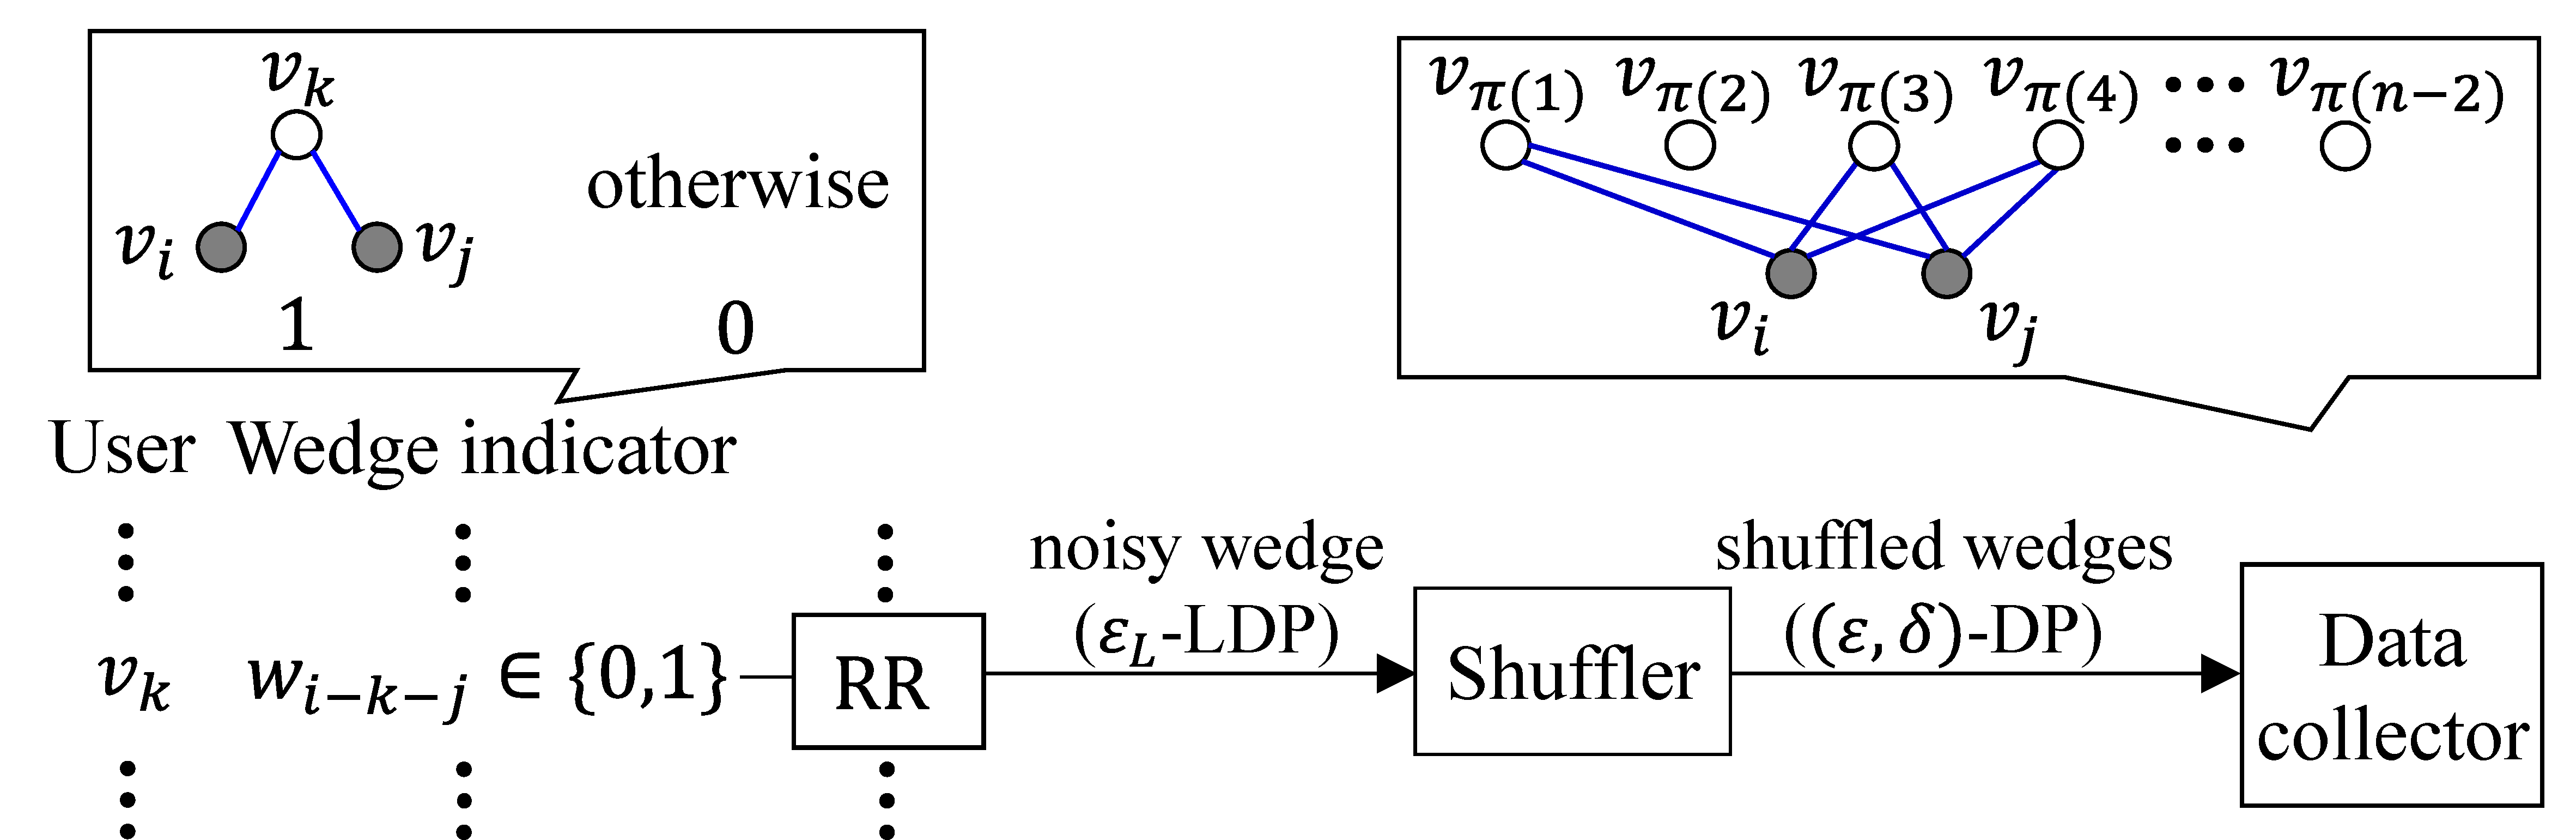
\includegraphics[width=0.99\linewidth]{fig/wedge_shuffle.pdf}
  \vspace{-2mm}
  \caption{Overview of wedge shuffling with inputs $v_i$ and $v_j$. 
  %(marked with gray).
  }
  \label{fig:wedge_shuffle}
\end{figure}

% \setlength{\algomargin}{5mm}
% \begin{algorithm}[t]
%   \SetAlgoLined
%   \KwData{Adjacency matrix $\bmA \in \{0,1\}^{n \times n}$, $\epsilon_L \in \nnreals$, user-pair $(v_i,v_j)$.}
%   \KwResult{Shuffled wedges $\{y_{\pi(k)} | k \in I_{-(i,j)}\}$.}
% %   \tcc{Set-up}
%   $I_{-(i,j)} \leftarrow [n]\setminus\{i,j\}$\;
% %   $\epsilon_L \leftarrow \texttt{LocalPrivacyBudget}(n,\epsilon,\delta)$\;
% %   \tcc{Users}
%   \ForEach{$k \in I_{-(i,j)}$}{
%     [$v_k$] $w_{i-k-j} \leftarrow a_{k,i} a_{k,j}$\;
%     [$v_k$] $y_k \leftarrow \calR_{\epsilon_L}^W(x)(w_{i-k-j})$\;
%     [$v_k$] Send $y_k$ to the shuffler\;
%   }
% %   \tcc{Shuffler}
%   [s] Sample a random permutation $\pi$ over $I_{-(i,j)}$\;
%   [s] Send $\{y_{\pi(k)} | k \in I_{-(i,j)}\}$ to the data collector\;
% %   \tcc{Data collector}
%   [d] \KwRet{$\{y_{\pi(k)} | k \in I_{-(i,j)}\}$}
%   \caption{Our wedge shuffle algorithm \AlgWS{}. 
%   [$v_k$], [s], and [d] represent that the process is run by user $v_i$, the shuffler, and the data collector, respectively. 
%   }\label{alg:WShuffle}
% \end{algorithm}

% To accurately count subgraphs such as triangles and 4-cycles, we propose a basic technique, which we call \textit{wedge shuffling}. 

% \smallskip
% \noindent{\textbf{Overview.}}~~
Figure ~\ref{fig:wedge_shuffle} shows the overview of our wedge shuffle technique. 
% First, we propose a basic technique, which we call wedge shuffling, to enable privacy amplification of graph data by shuffling. 
This technique calculates the number of wedges (two-hop paths) between 
% a specific user-pair $(v_i, v_j)$. 
a specific pair of users $v_i$ and $v_j$. 
%from user $v_i$ to $v_j$. 

% Algorithm~\ref{alg:WShuffle} shows our wedge shuffle algorithm. 
Specifically, 
% we consider the problem of counting triangles including a specific user-pair $(v_i, v_j)$ 
% and propose a wedge shuffle algorithm to accurately count them. 
given users $v_i$ and $v_j$, 
% our wedge shuffle algorithm calculates 
each of the remaining users $v_k$ ($k \ne i, j$) 
% \in [n]\setminus\{i,j\}$) 
calculates a \textit{wedge indicator} $w_{i-k-j} \in \{0,1\}$, 
which 
takes $1$ if and only if 
a wedge $v_i$-$v_k$-$v_j$ exists. 
Then, $v_k$ obfuscates $w_{i-k-j}$ using $\epsilon_L$-RR and sends it to the shuffler. 
The shuffler randomly shuffles the noisy wedges using a random permutation $\pi$ over $[n-2]$ 
% $[n]\setminus\{i,j\}$ 
to provide $(\epsilon, \delta)$-DP with $\epsilon \ll \epsilon_L$. 
Finally, the shuffler sends the shuffled wedges to the data collector. 
The only information available to the data collector is  the number of wedges from $v_i$ to $v_j$, i.e., the number of common friends of $v_i$ and $v_j$. 

Our wedge shuffling has two main features. 
First, 
% Because 
the wedge indicator $w_{i-k-j}$ is \textit{one-dimensional binary data}. 
Therefore, it can be sent with small noise and small $\epsilon$, unlike the $n$-dimensional neighbor list. 
For example, when $n=10^5$, $\delta=10^{-8}$, and $\epsilon=1$, the value of $\epsilon_L$ in (\ref{eq:shuffle_epsilon_f}) and (\ref{eq:shuffle_epsilon}) is $\epsilon_L = 5.44$. 
In this case, $\epsilon_L$-RR rarely flips $w_{i-k-j}$ -- the flip probability is $0.0043$. 
In other words, the shuffled wedges are almost free of noise. 

Second, the wedge is a main component of many subgraphs such as triangles, $k$-triangles \cite{Karwa_PVLDB11}, and 4-cycles. 
For example, a triangle consists of one wedge and one edge, e.g., $v_i-v_{\pi(3)}-v_j$ and $(v_i, v_j)$ in Figure ~\ref{fig:wedge_shuffle}. 
More generally, a $k$-triangle consists of $k$ triangles sharing one edge. 
Thus, it can be decomposed into $k$ wedges and one edge. 
A 4-cycle consists of two wedges, e.g., $v_i-v_{\pi(1)}-v_j$ and $v_i-v_{\pi(3)}-v_j$ in Figure ~\ref{fig:wedge_shuffle}. 
Because the shuffled wedges have little noise, we can accurately count these subgraphs based on wedge shuffling, compared to local algorithms in which all edges are noisy. 
% The other components can be sent from users to the data collector directly (or through the shuffler without shuffling) after adding LDP noise, e.g., by Warner's RR. 
% For example, if the data collector has a noisy edge between $v_i$ and $v_j$, it can count triangles including $(v_i, v_j)$. 
% Similarly, the data collector can count $k$-triangles that consist of $k$ triangles sharing $(v_i, v_j)$. 
% % Because the shuffled wedges have little noise, our wedge shuffling can significantly reduce the DP noise when compared to local algorithms. 
% Moreover, the data collector can count 4-cycles including $v_i$ and $v_j$ (e.g., $v_i-v_{\pi(1)}-v_j-v_{\pi(3)}-v_i$ in Figure ~\ref{fig:wedge_shuffle}) based only on the shuffled wedges. 
% Because the shuffled wedges have little noise, we can accurately count these subgraphs by sampling user-pairs and shuffling wedges. 

In this work, we focus on triangles and 4-cycles and 
present algorithms with upper bounds on the estimation error based on our wedge shuffle technique. 
% use our wedge shuffle technique for accurately counting them. 

% \smallskip
% \noindent{\textbf{Algorithm.}}~~Algorithm~\ref{alg:WShuffle} shows 

% \subsection{Algorithm}
% \label{sub:4cycle_algorithm}
% TBD

% \subsection{Theoretical Analysis}
% \label{sub:4cycle_theoretical}
% TBD
